\chapter{Methodology}
\label{chap:2}
\ChapterPageStuff{2}

\section{Preamble} The literature in \Cref{chap:1} is used for the method to create a logging mechanism that can capture user-based activity logs to improve software maintenance by analysing the obtained logs. The web-based application system on this logging mechanism will be implemented on is an energy management system for the mining industry.\par In \Cref{Ch2:LoggingMechanism} the methodology to create a logging mechanism to capture user-generated events is discussed for web-based applications. The different functional requirements and interfaces are discussed in this section \cite{Anish2015}.\par In \Cref{ch2:system_utilisation_analysis} the methodology is discussed to analyse these obtained logs to improve software maintenance.

\section{Logging mechanism}\label{Ch2:LoggingMechanism} The logging mechanism will need to meet the requirements discussed in \Cref{sec:EventLogging} to capture the required logs to apply system utilisation analysis on it. \Cref{fig:ch2_systemDesign} is the design for the logging mechanism to capture the user's activities. In this figure, the logging mechanism is split up into two functional requirements parts (F/R) which consist of the client and server functional requirements.\par Each functional requirement has an interface requirement that transfers the data from one interface to another interface. These interfaces are labeled as I/F in \Cref{fig:ch2_systemDesign}. The \Cref{fig:ch2_systemDesign} is the client interface (F/R 1) and the server interface (F/R 2) that forms the entire logging mechanism to capture the user-based activity logs.

\begin{figure}[!htb] % An h :here, t: top, b: bottom.
	\centering % cent the figure
	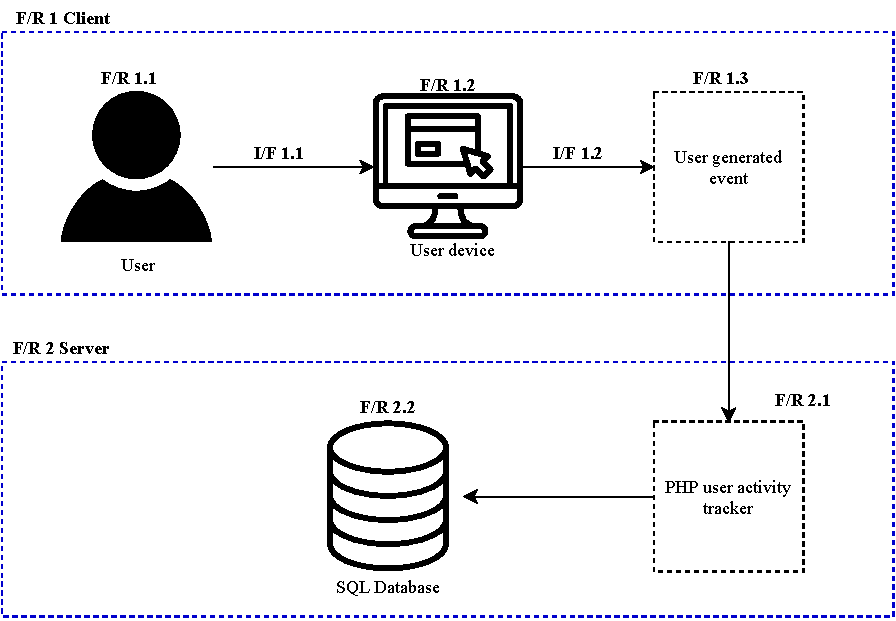
\includegraphics[width=0.9\textwidth]{Chapter2/SystemA_Architecture_Diagram/SystemA_Architecture_Diagram.pdf}
	\caption[Logging mechanism architecture design]
	{\textit{Logging mechanism architecture design}}\label{fig:ch2_systemDesign}
\end{figure}

\clearpage

\subsection{Clients functional requirements}

The client's functional requirements (F/R 1) are where the user-based activity is triggered. In \Cref{fig:ch2_systemDesign} the client interface consists of three main functional requirements. These interfaces in \Cref{tbl:ch2_clientFunctionalRequirements} parses the input from the user to create a basic user-based action that can be parsed be captured and parsed by the logging point to create a user-based log that is parsed onto the server for further processing. 

\begin{table}[!htb]
	\centering
	\caption[Client functional requirements]
	{\textit{Client functional requirements (F/R 1)}}
	\label{tbl:ch2_clientFunctionalRequirements}
	\begin{tabularx}{\textwidth}{|l|l|X|}
		\hline \textbf{Requirement ID} & \textbf{Name} & \textbf{Description} \\
		\hline F/R 1.1 & User & The user serves as the primary initiator of the user-based activity events.\\
		\hline F/R 1.2 & User's device & The device that the user uses to access the website from where the user-based activity events are generated.\\
		\hline F/R 1.3 & User-generated events & These are the captured user-based activity events that has been identified by the logging point and will be sent to the server.\\
		\hline
	\end{tabularx}
\end{table}

\subsection{Requirements for a user-based activity log}\label{sec:ch2_requirementsOfUAT}
The user is the initiator of the logging mechanism. Each action or event they trigger by interacting with the user interface on their device (F/R 1.2) can be a potential user-generated event. In
\Cref{tbl:ch2_requirementsForUserActivtyEvent} is the sub-requirements for the user (F/R 1.1) which the event log should fulfill to be classified as an user-based activity log.

\begin{table}[!htb]
	\centering
	\caption[Requirements for an event to be a user-based activity]
	{\textit{Requirements for an event to be a user-based activity}}
	\label{tbl:ch2_requirementsForUserActivtyEvent}
	\begin{tabularx}{\textwidth}{|l|X|}
		\hline \textbf{Requirement ID} & \textbf{Description}\\
		\hline F/R 1.1.1 & The event has to be triggered by the user interacting with the user interface using their device and not any other events that the system will self-initiate. The user needs to have interacted with the UI directly. This can also be validated by tracking if the user did interact with the UI from the HTML elements. \\
		\hline F/R 1.1.2 & The event must consists of different cases ($ca~ \epsilon~CA$ the cases consists of events) which are noteworthy to make the event log identifiable \cite{Slaninova2014}. \\
		\hline F/R 1.1.3 & For certain types of event logs for F/R 1.1.2, the user-generated event should have an origin from which the event took place. \\
		\hline F/R 1.1.4 & The event log should consist of attributes that expand the identity of the user-based activity. \\
		\hline F/R 1.1.5 & The event must have the user as the initiator or input for the user-based activity. This will exclude all events triggered by the system as the user did not directly start the event. \\
		\hline F/R 1.1.6 & Only use the first \textit{HTTP requests}\footnote{A \textbf{HTTP request} is made by a client, to a named host, which is located on a server. The request aims to access a resource on the server. \cite{IBM2021}.} that is sent to the server. \\ 
		\hline
	\end{tabularx}
\end{table}

Every interaction the user has with the user interface of the device to the software system can be seen as an event triggered by the user. Most of these events won't have a meaningful impact as they won't fulfill F/R 1.1.2 and F/R 1.1.4 in \Cref{tbl:ch2_requirementsForUserActivtyEvent}.\par For the user activity event to meet the requirement of 1.1.2 it has to have defined cases that describe the activity type of each event. These activity types form the basic criteria for which event can be parsed which significantly reduces the number of logs that will be obtained. This will ensure that the event logging process will produce quality user-based logs as discussed in \Cref{sec:ch1_loggingQuality}:

\begin{itemize}
	\item A basic structural complexity to simplify log parsing and development of the logging points in the system,
	\item Keep the logging consistent by not deviating from the defined cases, and
	\item Ensure that the event log's other attributes are complete and available to increase the accuracy and trustworthiness of the event logging when further system utilisation analysis needs to be done. 
\end{itemize}

\subsection{User activity types}\label{sec:ch2_userActivityTypes}
The user-activity logs will be split into three main event types as in \Cref{tbl:ch2_userActivityTypes}. The general user activity event type (F/R 1.2.3) will the be most common user activity event and be split up into different user activity events. This is determined by the need of what utilisation stage requires to analyse specific user activity events. 

\begin{table}[!htb]
	\centering
	\caption[User activity types]
	{\textit{User activity types}}
	\label{tbl:ch2_userActivityTypes}
	\begin{tabularx}{\textwidth}{|l|l|X|}
		\hline \textbf{Requirement ID} & \textbf{Activity Type} & \textbf{Description} \\
		\hline F/R 1.2.1 & Web page accessed & The user may navigate through different web pages in a session.\\
		\hline F/R 1.2.2 & Session changes & This is any user activities excluding F/R 1.2.1 that modifies the user's session:
		\begin{itemize}
			\item Logging into a Web application. Both Successful and failed attempted logins. This user-based activity may cause the log attributes that identify the user will be a NULL value as the user's session has not started yet to verify their identity,
			\item Ending their session through by logging out or declining to extend their session when it is about to expire,
			\item Modifying any session other relevant variables that can used in the utilasation analysis
		\end{itemize}\\
		\hline F/R 1.2.3 & General activity & Any events excluding the first two user-based activity types that the user initiates when they interact with the web page. Most of the user activity logs will
		have this event type.\\ 
		\hline
	\end{tabularx}
\end{table}

These user activity types can be further expanded in general activity (F/R 1.2.3) for analysis purposes. The general activity types will be different for each system based on what the system enables the user to do or what is needed for futher system utilisation analysis such as determining if the action the user triggered was to generate a report that they downloaded.

\subsection{Logging points}\label{sec:ch2_loggingPoints}
In \Cref{sec:ch1_loggignPoints} the logging points should be strategically placed in the software system to capture the log attributes for the user-based activity log. To meet the requirements of \Cref{tbl:ch2_requirementsForUserActivtyEvent} for a user-based activity the logging points should adhere to the logging points functional requirements of \Cref{tbl:ch2_loggingPointRequirement}.

\begin{table}[!htb]
	\centering
	\caption[Logging points requirements]
	{\textit{Logging points requirements}}
	\label{tbl:ch2_loggingPointRequirement}
	\begin{tabularx}{\textwidth}{|l|X|}
		\hline \textbf{Requirement ID} & \textbf{Description} \\
		\hline F/R 1.4.1 & The logging point should be placed where the user's interaction with the software system will send a \textit{request} back to the server.\\
		\hline F/R 1.4.2 & Each logging point should consistently capture the user-based activity as the activity is happening. \\
		\hline F/R 1.4.3 & Logging points should be globally complete to capture the user-based activities in the giving software system without too much modification between each point in the same
		software system. \\
		\hline F/R 1.4.4 & The logging points should not interfere with the rest of the system's operations, this would be slowing down the system by causing too much overhead in each \textit{request}
		that is being sent. \\
		\hline
	\end{tabularx}
\end{table}

The logging points can either be a single code segment or consist of multiple code segments in a software system that aims to capture user-based actions as they happen. Creating multiple logging points in a software environment will:

\begin{itemize}
	\item Increase complexity of the logging mechanism. Each point can be different from the other as it will need certain operations to capture the log,
	\item The consistency of the logging might differ and increase as the logging points increases in a software system. 
	\item The correctness of the logging will be impacted if the different changes in the logging point if the logging points are unable to consistently capture the user-based activity or extract all the needed attributes to complete the user-based log.
\end{itemize}

Creating a single logging point reduces the complexity and in most cases will improve the consistency and correctness of the user-based logs. In Web applications a globally defined logging point can be used in a modified \textit{AJAX request}\footnote{\textbf{AJAX} stands for Asynchronous JavaScript And XML. It uses an XMLHttpRequest object to communicate with servers that can send and receive information in various formats, including JSON, XML, HTML, and text files. \cite{Mozilla2022a}.} that will form the base template for all or most \textit{AJAX request} used in the software system as in \Cref{sec:ch2_webApplicationArchitecture}.\par The use of a single centralised logging point doesn't guarantee that the logging mechanism will perform more efficiently and accurately than using multiple logging mechanisms. Using a single logging point may have complexity issues when it needs to capture each user-based activity consistently with different cases.

\subsection{Log attributes}
The defined logging attributes in \Cref{tbl:ch2_keyLoggingAttributes} are the base attributes that form part of the main structure of the user-based event log. For web-based applications on the
client side, only some of these attributes can be obtained as the rest of the attributes can be resolved on the server side. The metadata (F/R 1.4.6) can consist of the request parameters that are
obtainable at the server side but any additional captured data can be added and sent to the server.

\begin{table}[!htb]
	\centering
	\caption[Key logging attributes]
	{\textit{Key logging attributes}}
	\label{tbl:ch2_keyLoggingAttributes}
	\begin{tabularx}{\textwidth}{|l|l|X|}
		\hline \textbf{Requirement ID} & \textbf{Logging point} & \textbf{Description} \\
		\hline F/R 1.4.1 & Identification number & The activity identification is an incremental number of the user-based event that is logged.\\
		\hline F/R 1.4.2 & Timestamp & This is the time the user initiated the user-based activity event. This will be the timestamp the log was written into the database as the log will be made before the rest of the intended \textit{HTTP request} is completed. \\
		\hline F/R 1.4.3 & Activity type & Each event can be classified into user-based types. This is the user-based activity types in \Cref{tbl:ch2_userActivityTypes}.\\
		\hline F/R 1.4.4 & User identification & Each user has a unique identification number that links the event to them if their session has been verified and can be obtained. Will not be available when the user tries to log in to the system as their session has not been set yet. \\
		\hline F/R 1.4.5 & Request origin & In web applications, there are always requests sent back to the server and will call the primary function to handle the request. This can be logged as either the file that the request is being sent to or the Webpage from which the request came. \\
		\hline F/R 1.4.6 & Metadata & The metadata of the event contains request parameters or other relevant request data of the event. This metadata adds more information about the user's activity.
		In \Cref{fig:Ch2_Metadata_Json_Example} is an example representation of the metadata that can be created for most user-based logs. Some of the event types may not have metadata added. \\
		\hline F/R 1.4.7 & Miscellaneous & These are any non-metadata attributes that can be consistently captured to be used in the utilisation analysis. They expand the characteristics of the obtained user-based log beyond the base attributes. \\ \hline
	\end{tabularx}
\end{table}

\clearpage

Each of these log attributes combined creates the base log from which key logging points can be created in the software system to capture the user-based activity logs in \Cref{tbl:ch2_keyLoggingAttributes}. The activity type (F/R 1.4.3) is can be assigned during the user-based activity identification phase with a default value and resolved to a new activity type based on metadata or other parameters by:

\begin{itemize}
	\item If it alters any of the session variables that are relevant to the system utilisation analysis,
	\item Access a certain part of the software system that needs all the user-based activities set to a certain type based on the nature of the procedures that need to be executed such as triggering a generation of a report that can be its user-based activity type.
	\item The activity type is also sorted by HTML element tags such as a button or textbox.
\end{itemize}

The metadata in \Cref{fig:Ch2_Metadata_Json_Example} is the possible extra parameters that can be obtained for the user-bade activity log. These parameters can either be captured at the client side by the logging point or can either be captured on the server side when the rest of the log's attributes are being obtained.

\begin{lstlisting}[style=json, caption={Metadata JSON}, label={fig:Ch2_Metadata_Json_Example}] 
	{ "RequestTarget" : "/Area4/Controller4/TestFunction",
		"RequestElementID" : "Button4",
		"RequestParameters": {
			"Parameter1": 4,
			"Parameter2": "Hello World!",
			"Parameter3": true
			"Parameter4": 40.404
			"Parameter5": {
				"Parameter6": "Car",
				"Parameter7" 160000.00
			}
		}		
	}
\end{lstlisting}

The metadata will need to store as a JSON string as it can be a complex object that doesn't have a set number of parameters. This complex object can have:

\begin{itemize}
	\item The \texttt{RequestTarget} parameter can be a file path for the \textit{Controller} or Webpage's absolute request path from where the user initiated the event. It also contains the function that is being called by the \textit{HTTP request}.
	\item The \texttt{RequestElementID} is the HTML element which the user interacted with that cause the user-based activity. This can be used as another validation that the event was caused by the user. Some of the user-based activities can be set to some of these HTML element controls by getting the HTML element tag.
	\item The \texttt{RequestParameters} is all the parameters in the \textit{HTTP request} that can be serialize into a JSON string. This can be used to determine what the user tried to do by using this input for the specific function which is used for F/R 1.1.6 in \Cref{tbl:ch2_requirementsForUserActivtyEvent}.
\end{itemize}

\subsection{Web application architecture}\label{sec:ch2_webApplicationArchitecture}
To determine the user activity types for a Web application, the Web application's architecture will be a factor in the logging mechanism. Web applications consist mostly of HTML, JavaScript and CSS programming languages. The Model-View-Controller (MVC) architecture is mostly used for web-based applications using that programming language \cite{Jailia2016}. The MVC architecture in \Cref{fig:ch2_flowMVC_Architecture} consists of 3 basic parts which are the \cite{Jailia2016}:

\begin{itemize}
	\item \textit{Model:} Is the representation of the records in the database which also interacts with the database through a database access layer or service manipulating the data by using the CRUD operations:
	\begin{itemize}
		\item \textit{create} operation that adds new data,
		\item \textit{read} operation that gets the data from the database,
		\item \textit{update} operation that modifies the existing data,
		\item \textit{delete} operation that removes data.
	\end{itemize}
	\item \textit{Controller:} Is operates both the \textit{View} and \textit{Model} and serves as the connection between the user and the system by controlling the data flow of the \textit{Model} and
	\textit{View}.
	\item \textit{View:} This shows the results of the data contained in the \textit{Model} and enables the user to manipulate the data. The user will only interact with this part of the Web application.
\end{itemize}

\begin{figure}[!htb] % An h :here, t: top, b: bottom.
	\centering % cent the figure
	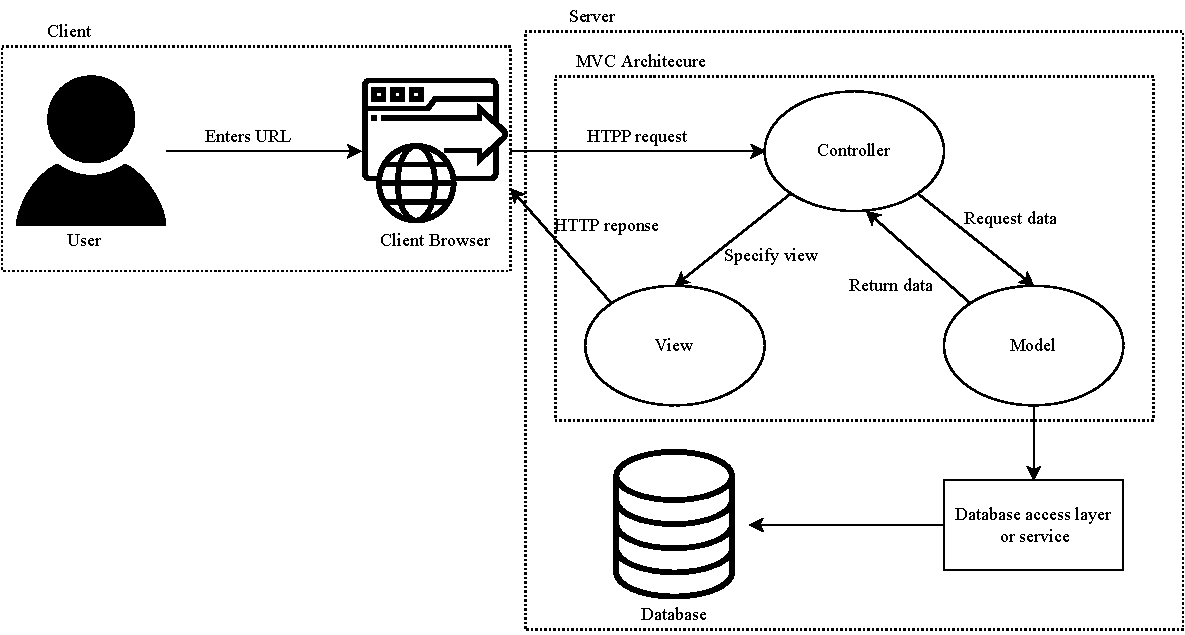
\includegraphics[width=0.9\textwidth]{Chapter2/Flow_MVC_Architecture/Flow_MVC_Architecture.pdf}
	\caption[MVC architecture for most web-based applications]
	{\textit{MVC architecture for most web-based applications \cite{Gu2010}}}\label{fig:ch2_flowMVC_Architecture}
\end{figure}

In \Cref{fig:ch2_flowMVC_Architecture} is the MVC architecture equivalent representation of \Cref{fig:ch2_systemDesign} where the data flow is shown of the MVC architecture. The user interacts with the Web application through their browser which will send a \textit{HTTP requests} to the \textit{Controller} and receive a \textit{HTTP response}\footnote{An \textbf{HTTP response} is made by a server to a client. The response aims to provide the client with the resource it requested, inform the client that the action it requested has been carried out; or else inform the client that an error occurred in processing its request. \cite{IBM2021a}.} from the \textit{View}.The \textit{Controller} will request and return the data to the \textit{Model} which interacts with the database access layer or service to do the \textit{create}, \textit{update} and \textit{delete} operations.\par To classify any interaction between the user (F/R 1) and server (F/R 2) to fulfill the functional requirements of \Cref{tbl:ch2_requirementsForUserActivtyEvent} only the \textit{HTTP request} are used for the logging points in \Cref{sec:ch2_loggingPoints} as it:

\begin{itemize}
	\item Meet the F/R 1.1.1 and F/R 1.1.5 as the user will interact with the \textit{View} to modify the data which needs to send back an \textit{HTTP request} to process the data on the \textit{Controller}.
	\item User activity types can be assigned for different scenarios that the user triggers when the request is being sent. 
	\item Any additional metadata can be sent with the \textit{request header}\footnote{A \textbf{request header} is an HTTP header that can be used in an HTTP request to provide information about the request context so that the server can tailor the response. For example, the Accept-$\ast$ headers indicate the allowed and preferred formats of the response. \cite{Mozilla2022}.} of the \textit{HTTP request}. This will reduce the overhead added by the logging mechanism by not sending additional \textit{HTTP request} each time back to the server when a user-based activity has been identified.
\end{itemize}

Most Web applications will make of use JavaScript to control the content of the page that is being displayed to the user. The primary method would be making use of an \textit{AJAX request} to communicate with the server to fulfill the user's action.\par The \textit{AJAX request} has some key features that will enable the logging points discussed in \Cref{sec:ch2_loggingPoints}

\begin{figure}[!htb]
	\centering
	\begin{lstlisting} 
		$.ajax({
			url: "https://fiddle.jshell.net/favicon.png",
			beforeSend: function (xhr) {
				xhr.overrideMimeType("text/plain; charset=x-user-defined");
			}
		}).done(function (data) {
			if (console && console.log) {
				console.log("Sample of data:", data.slice(0, 100));
			}
		});
	\end{lstlisting}
	\caption[AJAX request example]
	{\textit{AJAX request example}}\label{fig:ch2_ajaxBeforesend}
\end{figure}

\clearpage

\subsection{Client functional requirements interaction}
\par In \Cref{fig:ch2_user_based_actvity_classification} is the complete process of the user interacting with the UI to trigger a user-based activity event to be logged later for the client's functional requirements. It starts with the user interacting with the user interface. The potential user activity needs to meet the first requirement (F/R 1.1.1) of \Cref{tbl:ch2_requirementsForUserActivtyEvent} or else it should be not be logged. The default activity type is set to general activity (F/R 1.2.3) until it is further processed later in the logging mechanism.\par If the activity has any additional metadata such as the request parameters, it will also be logged. The other metadata can also be captured in this stage from the client side like the element that the user clicked on to start the event.

\begin{figure}[!htb] % An h :here, t: top, b: bottom.
	\centering % cent the figure
	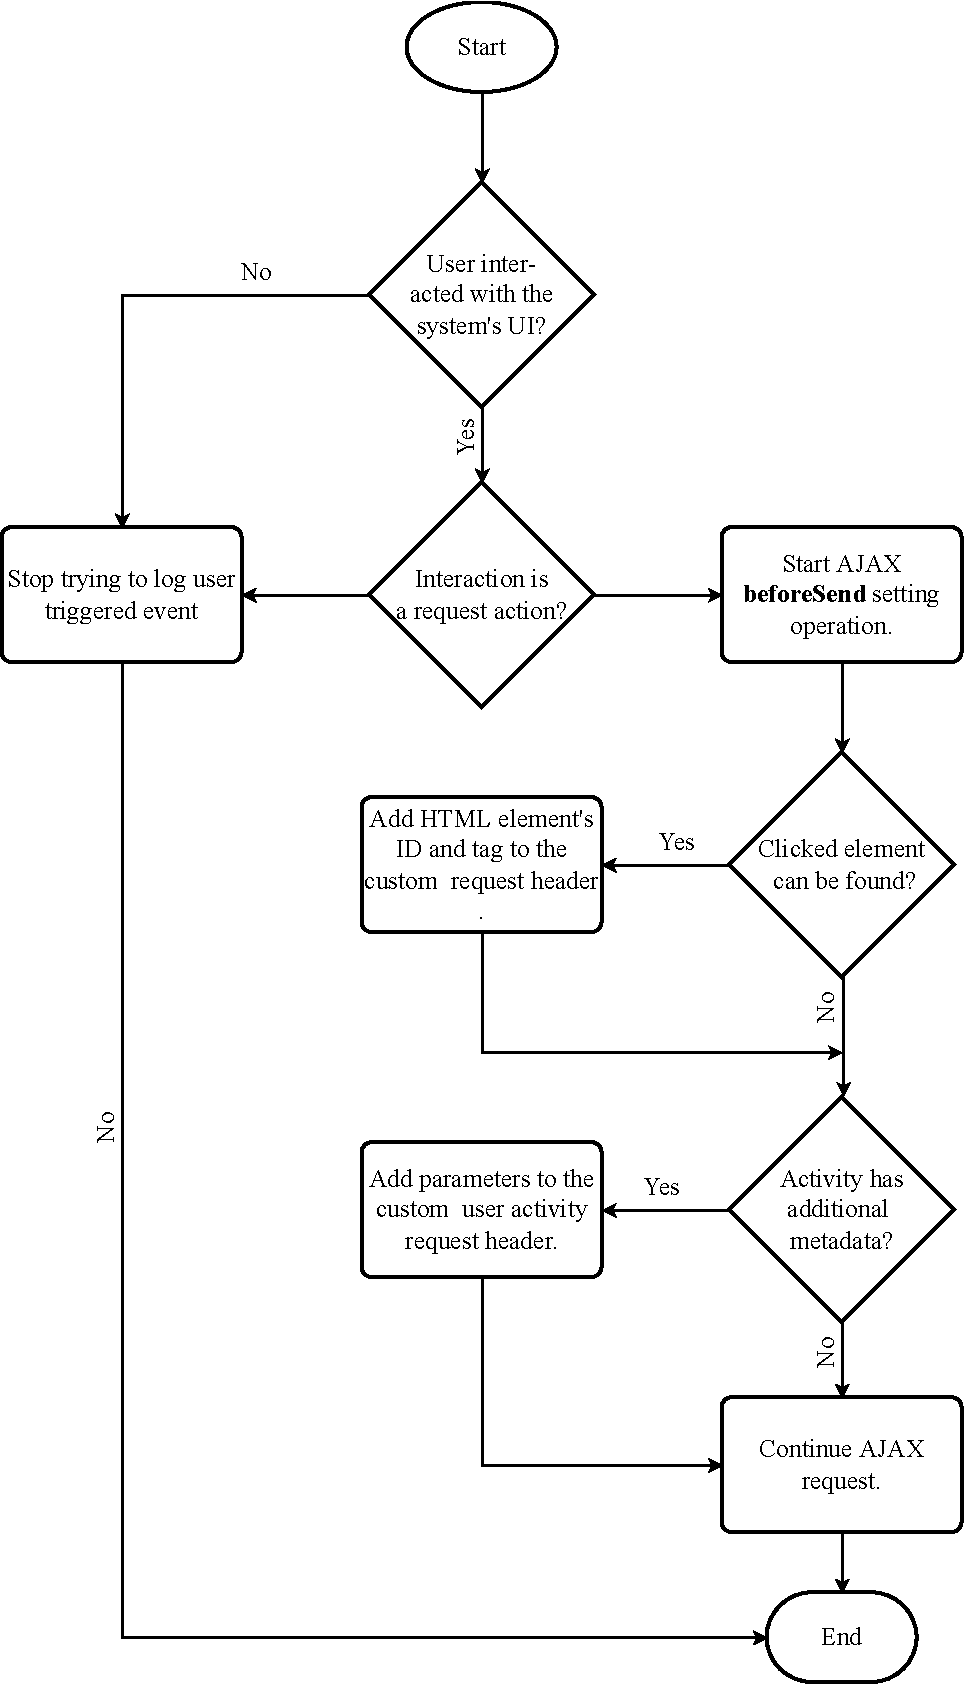
\includegraphics[width=0.6\textwidth]{Chapter2/client_functional_requirement_flow_diagram/client_functional_requirement_flow_diagram.pdf}
	\caption[User-based activity log classification flow diagram]
	{\textit{User-based activity log classification flow diagram}}\label{fig:ch2_user_based_actvity_classification}
\end{figure}

\clearpage

\subsection{Server's functional requirements}
The server functional requirements in \Cref{tbl:Ch2_Server_Functional_Requirements} for \Cref{fig:ch2_systemDesign} is the rest of the logging mechanism. At this stage, the obtained user-generated event of \Cref{fig:ch2_user_based_actvity_classification} will be attempted to be completed into a user-based activity log and stored in a database.

\begin{table}[!htb]
	\centering
	\caption[Server functional requirements]
	{\textit{Server functional requirements (F/R 2)}}
	\label{tbl:Ch2_Server_Functional_Requirements}
	\begin{tabularx}{\textwidth}{|l|l|X|}
		\hline \textbf{Requirement ID} & \textbf{Name} & \textbf{Description} \\
		\hline F/R 2.1 & User activity logger & The key logging points are used to capture and create the user-based event log that will be stored in a database.\\
		\hline F/R 2.2 & Database & The event log is stored in a database until it is needed for further analysis.\\
		\hline
	\end{tabularx}
\end{table}

The interfaces in \Cref{tbl:ch2_serverInterfaceRequirements} for the client functional requirement (F/R 2) is to obtain the base log from the client functional requirement (F/R 1) and finally store the completed log into a database.

\begin{table}[!htb]
	\centering
	\caption[Server interface requirements]
	{\textit{Server interface requirements for F/R 2}}
	\label{tbl:ch2_serverInterfaceRequirements}
	\begin{tabularx}{\textwidth}{|l|l|X|}
		\hline \textbf{Requirement ID} & \textbf{Name} & \textbf{Description} \\
		\hline I/F 2.1 & Log parsing to server & The captured log is parsed onto the server for further processing of the captured user-generated event.\\
		\hline I/F 2.2 & Store in database & The event log is sent to a database for storing.\\
		\hline
	\end{tabularx}
\end{table}

\begin{figure}[!htb]
	\centering
	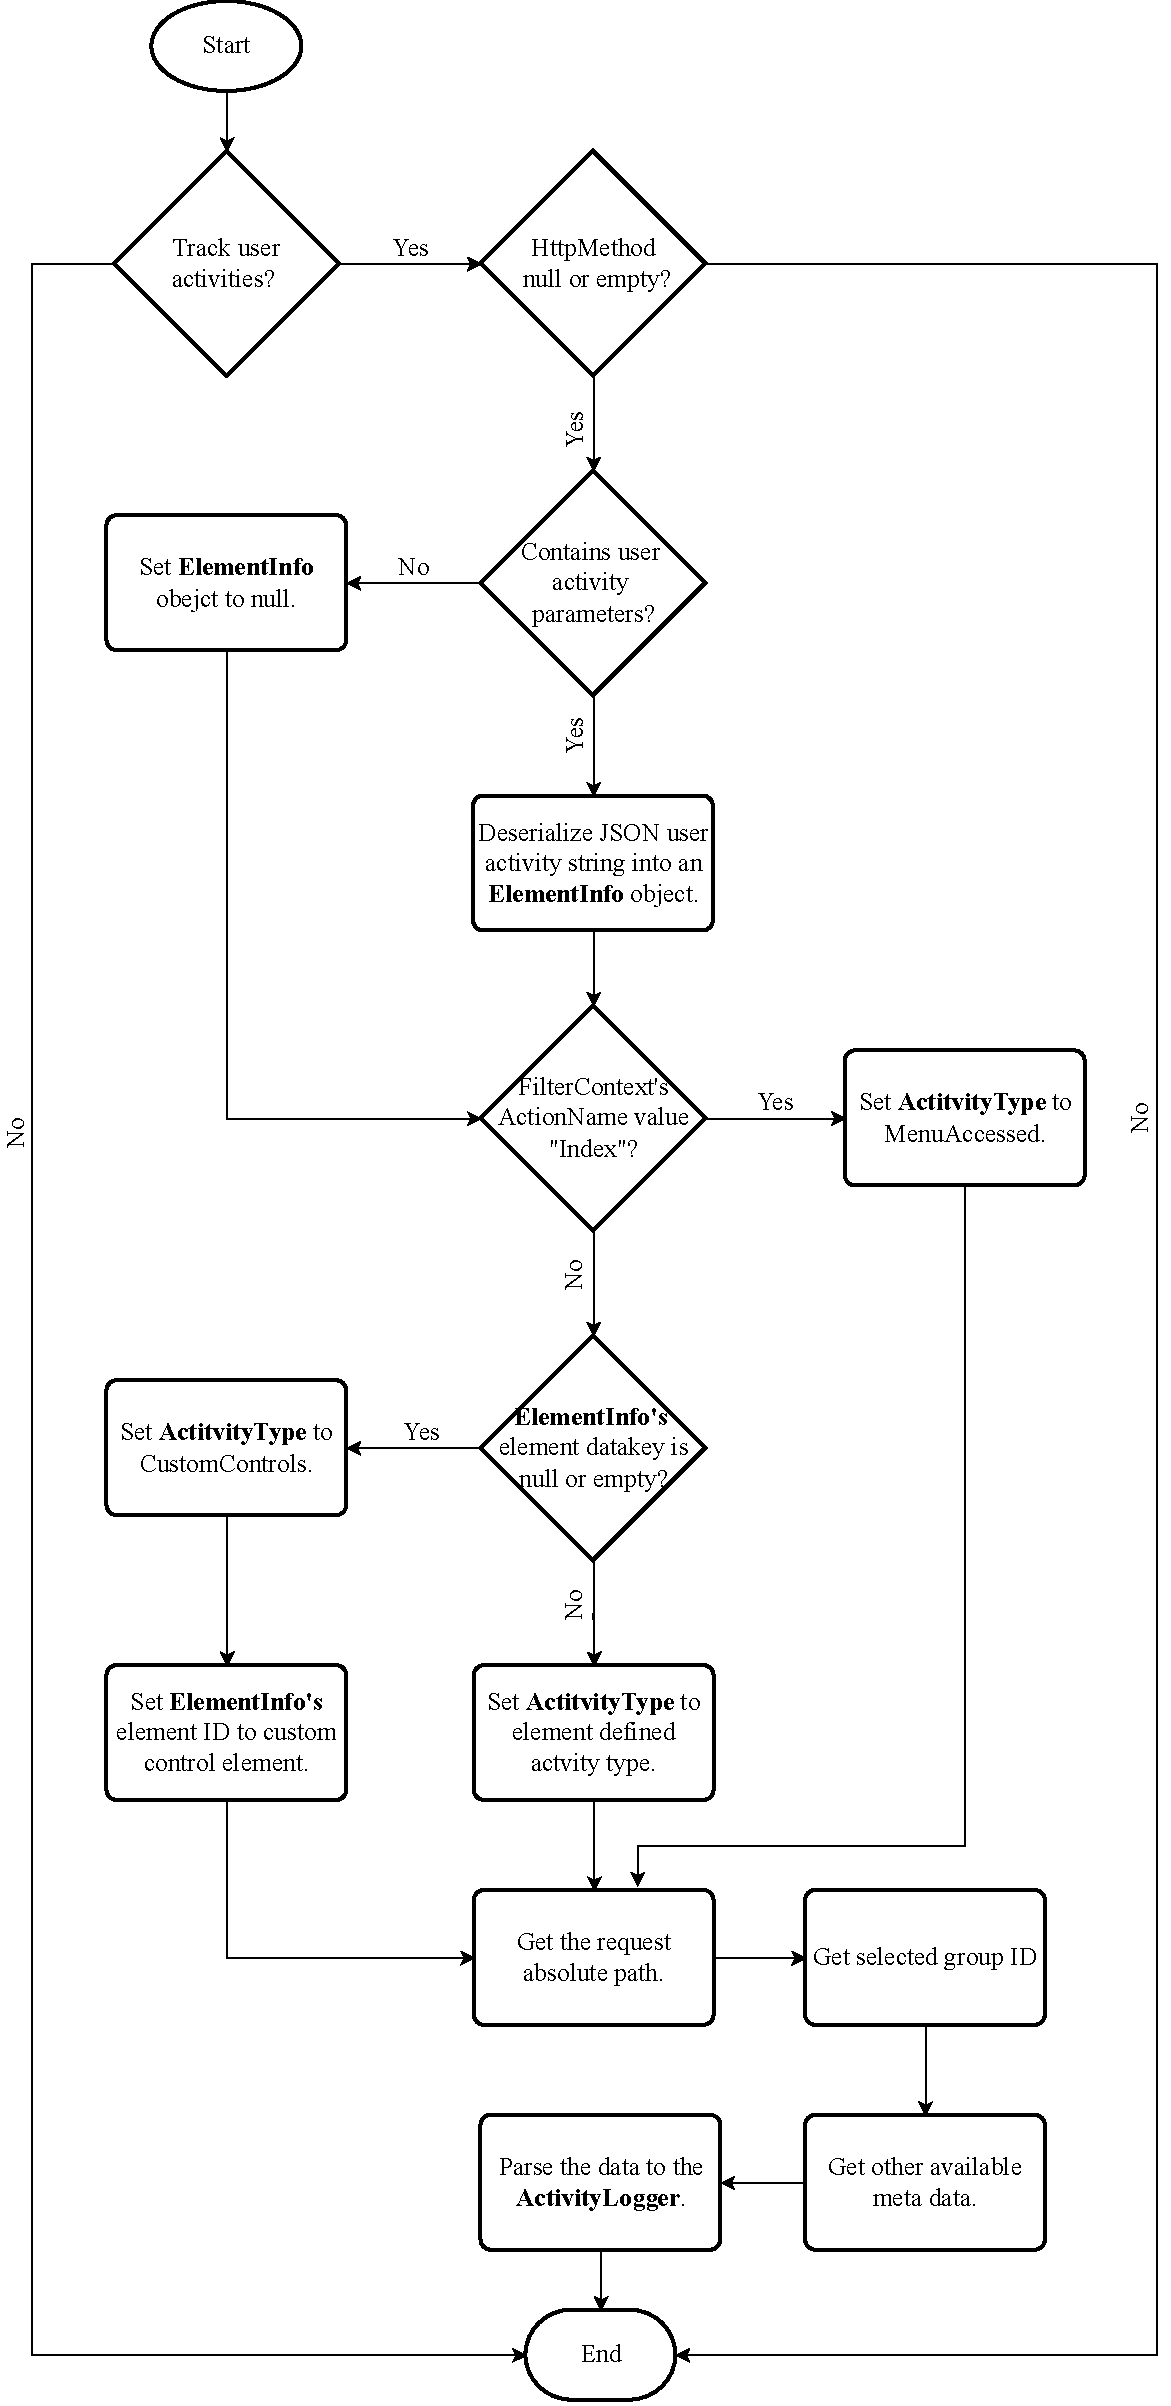
\includegraphics[width=0.7\textwidth]{Chapter2/SystemB_FilterContext/SystemB_FilterContext.pdf}
	\caption[System B event classification]
	{\textit{System B event classification flow diagram}}\label{fig:ch2_loggingParse}
\end{figure}

\begin{figure}[!htb] % An h :here, t: top, b: bottom.
	\centering % cent the figure
	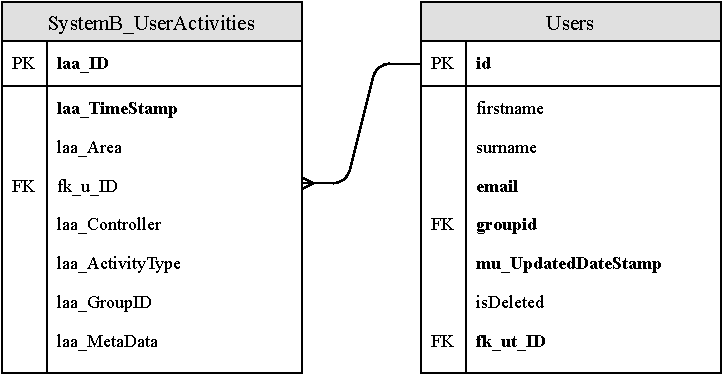
\includegraphics[width=0.99\textwidth]{Chapter2/SystemB_ERD_Basic/SystemB_ERD_Basic.pdf}
	\caption[ERD of user activities]
	{\textit{ERD of the user activities}}\label{fig:ch2_erdOfEventLogs}
\end{figure}

\begin{table}[!htb]
	\centering
	\small
	\caption[System B user activities table]
	{\textit{System B user activities table}}
	\label{tbl:ch2_SQLLoggingTable}
	\begin{tabularx}{\textwidth}{|l|l|X|}
		\hline \textbf{Column Name} & \textbf{SQL Data Type} & \textbf{Description} \\
		\hline \textbf{ActivityID} & INT(11) & The activity identification is an incremental number of the event that is logged.\\
		\hline \textbf{Timestamp} & DATETIME & This is the time which the event took place.\\
		\hline \textbf{ActivityType} & ENUM & Each event that the user initiate has an activity type as in \Cref{tbl:Ch2_SystemB_ActivityTypes}. This activity type is dependent if the controller's called method is the index action or based on the HTML element that is part of the meta data. \\
		\hline \textbf{UserID} & INT(4) & Each user has a unique identifier which is a numerical identification number that is foreign key reference to the User table. \\
		\hline \textbf{Area} & VARCHAR(45) & This information is logged to track user activities per Area that represents different software systems that the user can use. \\
		\hline \textbf{Controller} & TEXT & Each event will point back to an controller that process the request. \\
		\hline \textbf{GroupID} & INT(4) & This foreign key reference to the Group table is contract groups identification number. \\
		\hline \textbf{MetaData} & JSON & The meta data of the event contains request parameters, the HTML element from which the request is initiated and other relevant request data of the event. This can also be other meta data is important to get that adds more information about the user's activity using certain controls on System B as in \Cref{fig:CH2_SystemBMetaData}. \\
		\hline
	\end{tabularx}
\end{table}

\clearpage

\subsection{Database interaction of the logging mechanism}\label{sec:ch2_databaseInteraction}

In \Cref{fig:ch2_Dash_PHP_Flow,fig:ch2_DetailView_Flow} the user-generated event is captured with additional parameters that may exist with the captured event. The next process in \Cref{fig:CH2_SystemA_DB_Interaction_FlowDiagram} is save the generated user activity log in a database.\par \Cref{fig:CH2_SystemA_DB_Interaction_FlowDiagram} is the process which the logging mechanism will create a log entry by first initialising the SQL database connection. The last parameter needed to complete the requirements of the logging points in \Cref{tbl:Ch2_System_A_Logging_Points} is the user's identification. This is obtained from the user's session that contains the user's ID number that is assigned in the Users table.\par The ActivityParameters from  \Cref{fig:ch2_Dash_PHP_Flow,fig:ch2_DetailView_Flow} are encoded as a JSON string to be saved in the RequestParameters column. After all the parameters are converted to correct format the SQL query created and executed to save the log entry in the SystemA\_UserActivities table of \Cref{fig:Ch2_SystemA_Basic_ERD}.

\begin{figure}[!htb] % An h :here, t: top, b: bottom.
	\centering % cent the figure
	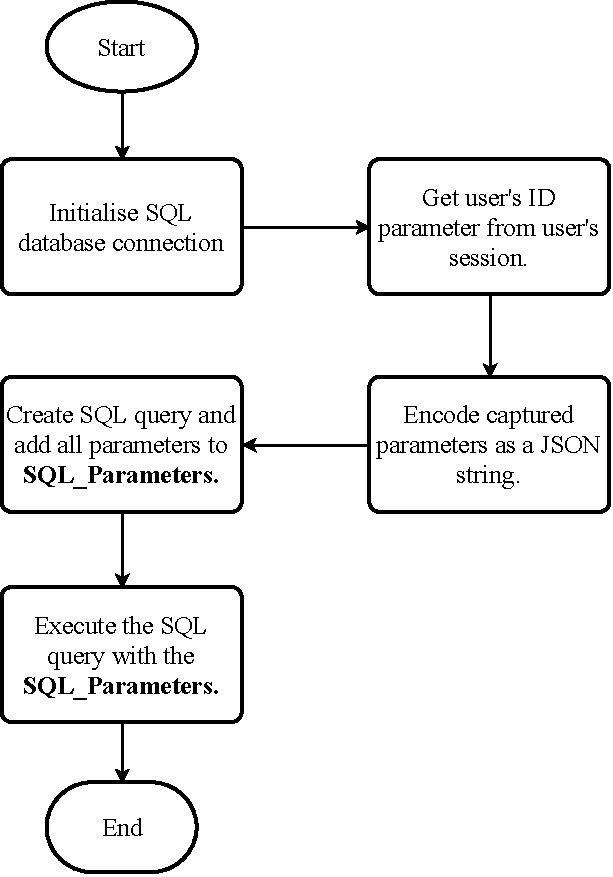
\includegraphics[width=0.5\textwidth]{Chapter2/SystemA_ActivityTracker/SystemA_ActivityTracker.pdf}
	\caption[User activity logging mechanism database interaction]
	{\textit{User activity logging mechanism database interaction}}\label{fig:ch2_databaseInteraction}
\end{figure}

\section{System utilisation analysis}\label{ch2:system_utilisation_analysis}

\section{Integration}

\section{Conclusion}